\chapter{Methodology}
Here we describe the selected algorithms and their parameters in detail. We also discuss the nature of the benchmarks and real world data, giving a summary of the range of tests to be performed. 

\section{Selected Algorithms}
\subsection{Tasgin-Bingol}
One of the earliest implementations of a genetic algorithm for the network clustering problem \cite{Tasgin2006}, Tasgin and Bingol's approach is an example of one of the more naive approaches. Each individual is represented as an array of size $n$, each index corresponding to a node of the input graph. The population is initialized with a random walk over the graph. . It utilizes modularity as its fitness function. Its mutation operator is simple. For the selected node $i$, select a member of $\Gamma(i)$, and set $i$ to be in its community.

The table \ref{table:1} is an example of referenced \LaTeX elements.

\begin{table}[h!]
	\centering
	\begin{tabular}{| c | c | c | c | c |}
		\hline
		Population Size & Generations & Crossover Rate & Mutation Rate  & Cleaning Rate \\ [0.5ex] 
		\hline
		1 & 6 & 87837 & 787 & 6  \\ 

		\hline
	\end{tabular}
	\caption{Tasgin-Bingol's default parameters}
	\label{table:1}
\end{table}

The



\subsection{GA-Net}


\cite{Pizzuti2008}
\begin{table}[h!]
	\centering
	\begin{tabular}{| c | c | c | c | c |}
		\hline
		Population Size & Generations & Crossover Rate & Mutation Rate  & Cleaning Rate \\ [0.5ex] 
		\hline
		1 & 6 & 87837 & 787 & 6  \\ 
		
		\hline
	\end{tabular}
	\caption{GA-Net's default parameters}
	\label{table:1}
\end{table}


\subsection{GACD}
\cite{Shi2009}
\begin{table}[h!]
	\centering
	\begin{tabular}{| c | c | c | c | c |}
		\hline
		Population Size & Generations & Crossover Rate & Mutation Rate  & Cleaning Rate \\ [0.5ex] 
		\hline
		1 & 6 & 87837 & 787 & 6  \\ 
		
		\hline
	\end{tabular}
	\caption{GACD's default parameters}
	\label{table:1}
\end{table}


\subsection{GALS}
\cite{liu2013genetic}
\begin{table}[h!]
	\centering
	\begin{tabular}{| c | c | c |}
		\hline
		Population Size & Generations  & a \\ [0.5ex] 
		\hline
		1 & 6 & a \\ 
		
		\hline
	\end{tabular}
	\caption{GALS' default parameters}
	\label{table:1}
\end{table}


\section{The Girvan-Newman Benchmark}

Girvan and Newman introduce a benchmark which is a special case of the planted $\ell$-partition model\cite{Girvan2002}. The graph is generated by creating 128 nodes, divided into 4 equally sized communities. Each node has an expected degree of 16. By setting the expected $k_{in}$ and $k_{out}$, the difficulty of discerning the partition can be tuned. With an expected $k_{out} < 8$, the communities are strongly defined. It should be expected that a well defined method should discern the structure with a fair degree of accuracy. 

The GN benchmarks limited size makes it an excellent model candidate for testing algorithms in early stages for the ability to detect loosely connected communities, but may not demonstrate the performance of a method when scaled\cite{Yang2016}.


\section{The LFR Benchmark}



\begin{tabular}{|c|}
	\hline 
	Number of Nodes \\ 
	\hline 
	Maximum Degree \\ 
	\hline 
\end{tabular} 

\cite{Lancichinetti2008}


\section{Benchmark Generator}
All synthetic networks were created using Andrea Lancichinetti's benchmark generation applications 

\section{Real World Data}
\subsection{Zachary's Karate Club}
Zachary's Karate Club \cite{Zachary1977} is one of the most widely used networks used to show an algorithm can effectively identify a set of communities. The graph shows the reported relationships between members of a martial arts club, after a schism was formed by a conflict between the lead instructor and the owner of the club. Though small, the graph shows the expected power law of degree distribution for 

\begin{figure}[!htb]
	\begin{center}
		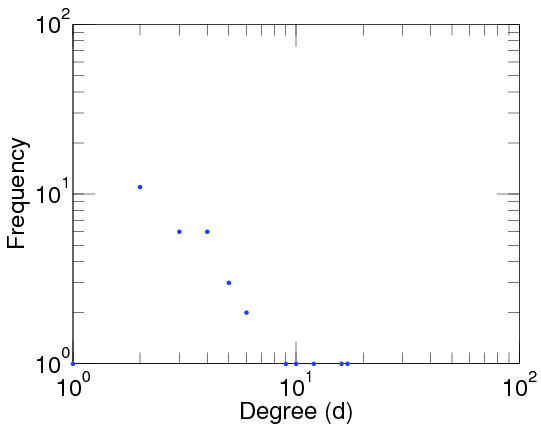
\includegraphics[scale=.5]{images/zachary_degree_dist.png}
	\end{center}
	\caption{Degree distribution of the karate club network\cite{Kunegis2013}}
	\label{logo}
\end{figure}

\subsection{Dolphins}
shibba shabba
\cite{Lusseau2003}
\begin{figure}[!htb]
	\begin{center}
		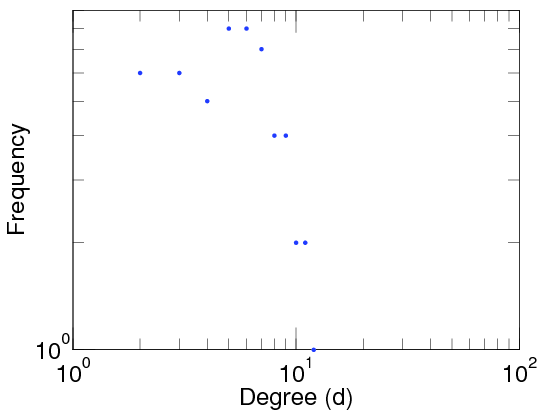
\includegraphics[scale=.5]{images/dolphins_degree_dist.png}
	\end{center}
	\caption{Degree distribution of the Dolphins network\cite{Kunegis2013}}
	\label{logo}
\end{figure}

blabba blabba

\subsection{College Football}

\cite{Girvan2002}
\begin{figure}[!htb]
	\begin{center}
		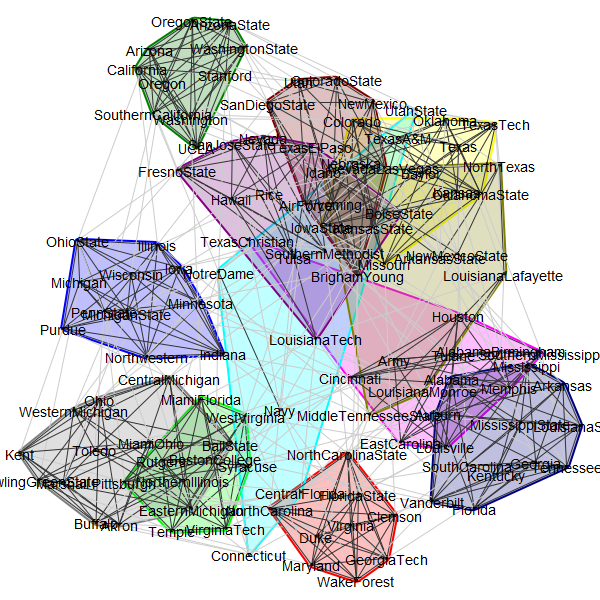
\includegraphics[scale=.5]{images/football.png}
	\end{center}
	\caption{The College Football network, with conferences grouped as communities}
	\label{logo}
\end{figure}


\subsection{Political Blogs}
\cite{Adamic2005}
asdasd


\section{Experiment Description}
The goal of this analysis is to compare the performance of the selected algorithms on a sufficient variety of networks, with sufficient complexity. The collection of generated and real world networks has been selected to reflect other comparative studies, and to extend the observations made in the literature proposing the algorithms. These networks come with ground truth, describing the community structure as it was generated, in the case of the synthetic networks, or as it is generally accepted when using real world data.

When comparing the generated community partitions, we use several measures

\subsection{Variation of Information}
\cite{Marina2007}

\subsection{Normalized Mutual Information}
The Normalized Mutual Information (NMI) of a community partition 

\subsection{Rand and Adjusted Rand Index}
\cite{rand1971}


\section{Comparing Performance}

The evaluation of algorithm performance, relative to set of different algorithms is a problem for statistical anlysis tools. Througho
